%% Beispiel-Präsentation mit LaTeX Beamer im KIT-Design
%% entsprechend den Gestaltungsrichtlinien vom 1. August 2020
%%
%% Siehe https://sdqweb.ipd.kit.edu/wiki/Dokumentvorlagen

%% Beispiel-Präsentation
\documentclass[en]{sdqbeamer} 
\usepackage{graphicx}
 
%% Titelbild
\titleimage{banner_2020_kit}

%% Gruppenlogo
\grouplogo{logo_empty.jpg} 

%% Gruppenname und Breite (Standard: 50 mm)
\groupname{}
%\groupnamewidth{50mm}

% Beginn der Präsentation

\title[Simple Prediction Intervals]{Simple and Transparent Macroeconomic Prediction Intervals}
\subtitle{} 
\author[Friederike Becker, Fabian Krüger, Melanie Schienle]{Friederike Becker, Fabian Krüger, Melanie Schienle}

\date[28.\,9.\,2023]{September 28, 2023}

% Literatur 
 
\usepackage[citestyle=authoryear,bibstyle=numeric,hyperref,backend=biber]{biblatex}
\addbibresource{presentation.bib}
\bibhang1em

\begin{document}
\setbeamertemplate{caption}{\raggedright\insertcaption\par}
 
%Titelseite
\KITtitleframe

%Inhaltsverzeichnis
\begin{frame}{Overview}
\tableofcontents
\end{frame}

\section{Setting}


%\subsection{Fixed-Event forecasting in Economics}
\begin{frame}{An economist's favorite pastime}
	\begin{itemize}
	    \item various institutions issue forecasts for annual macroeconomic targets
     \begin{itemize}
        \item most prominent targets: (real) GDP growth and inflation
        \item for Germany, sources are (among others) the Bundesbank, the ifo institute, the OECD
         \item fixed-event forecasts: target date is fixed, forecast date is not
     \end{itemize}
     \item forecasts are often disseminated widely
     \begin{itemize}
         \item extensive media coverage, influence on political discussions
         \item relevant for real-world outcomes (public budget planning, collective bargaining)
     \end{itemize}
	\end{itemize}
\end{frame}

\begin{frame}[t]{Can we really be that sure?}

\begin{columns}
\begin{column}{0.4\textwidth}
   	\begin{itemize}
         \item usual practice: issue point forecasts only
         \begin{itemize}
	    \item uncertainty is at best acknowledged, rarely quantified
	\end{itemize}
        %\item media reception often fixated on zero
        \item forecasts of different horizons are often left uncontextualized
        \item distributional forecasts supposedly would require extra modeling effort
    \end{itemize}
    \vspace{2cm}
\end{column}
\begin{column}{0.6\textwidth}
    \begin{figure}
        \centering
        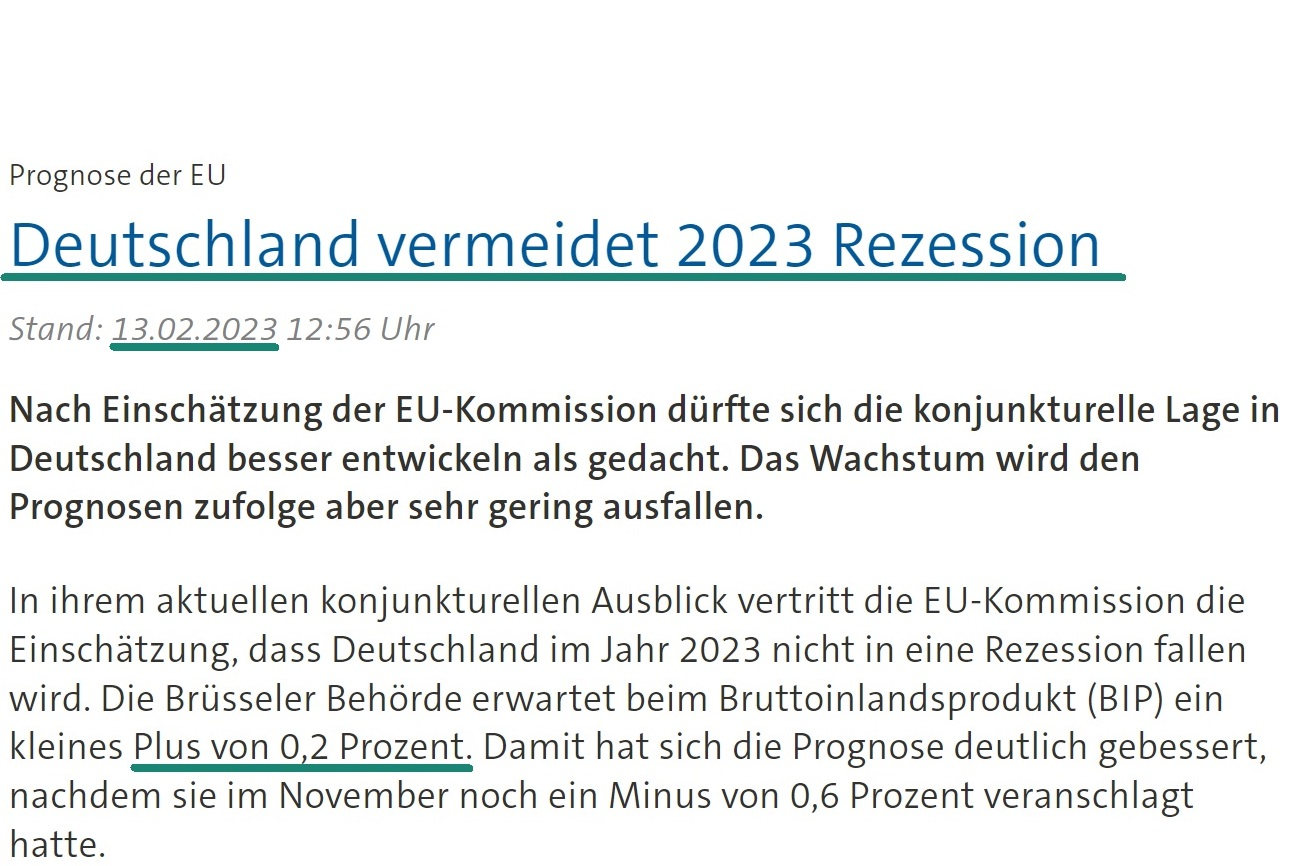
\includegraphics[width=0.8\textwidth]{figures/recession_light_underlined_green_smaller_date.jpg} 
        \caption{Source: tagesschau.de}
        \label{fig:enter-label}
    \end{figure}     
\end{column}
\end{columns}
\end{frame}

\begin{frame}[t]{Contributions of this work}
\begin{itemize}
    \item simple and transparent method of attaching prediction intervals 
\item show that attaching distributional forecasts to an existing
\item evaluate on years 1999-2021
\end{itemize}
\end{frame}

% \begin{flushright}
% 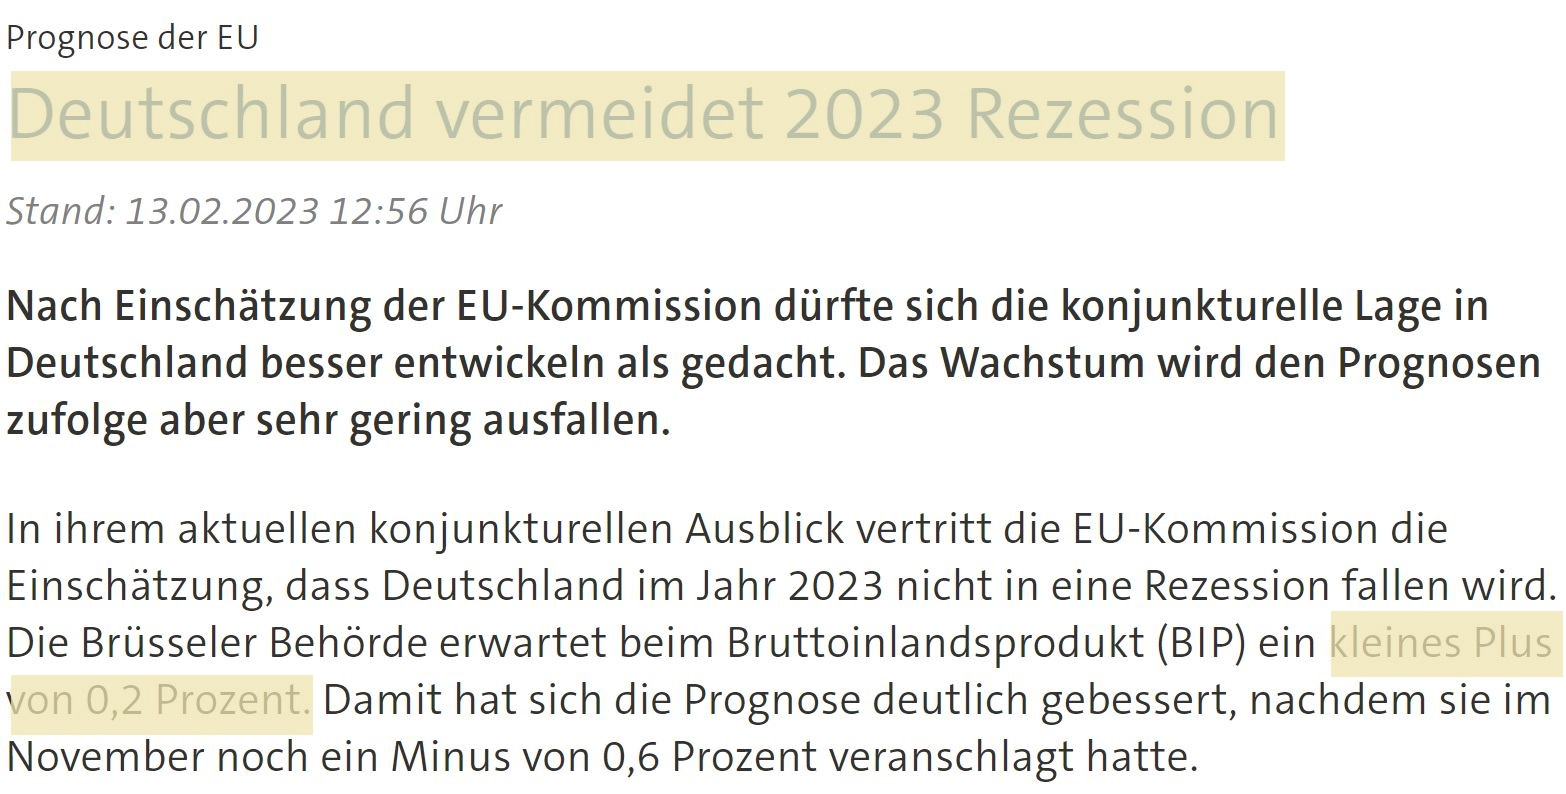
\includegraphics[width = 8cm]{figures/recession_light.JPG}    
% \end{flushright}
   
%\subsection{Data Source: IMF World Economic Outlook}
\begin{frame}{Data Source: IMF World Economic Outlook}
	\begin{itemize}
		\item survey by the IMF staff, published bi-annually
		\begin{itemize}
            \item contains forecasts with up to 6 years horizon and historic truth values
		    \item publication in April (horizon for current year $\approx$ 8 months) and in October ($\approx$ 2 months)
		\end{itemize}
    \item publicly available publication
    \item targets: real GDP growth and CPI inflation 
    \item available since 1990, giving $\sim$30 years of forecast-truth pairs per country and forecast horizon
    \item forecasts for G7 countries are (nearly) uninterrupted
    \begin{itemize}
        \item forecasts for 196 countries in total are available
    \end{itemize}
	\end{itemize}
\end{frame}

\section{Methods}
\begin{frame}{Methods}
We apply an attractively simple and cheap method. For a given country and target:
\begin{itemize}
    \item given forecasts $\hat{y}_{t, h}$ and the realized true values $y_{t}$ ...
    \begin{itemize}
        \item for target year $t$, horizon $h$
    \end{itemize}
    \item ... construct sets $\mathcal{E}_{t, h} = \{\hat{e}_{t^*, h}  | t-9 \leq t^* < t \}$, containing the last nine forecast errors
    \begin{itemize}
        \item based on \textit{absolute} errors $\hat{e} = |y_{t} - \hat{y}_{t, h}| $
        \item sets are stratified by country, target and horizon
    \end{itemize}
    \item for $\alpha \in \{0.5, 0.8\}$, compute $q^{\alpha}_{t, h} =  Q\left(\mathcal{E}_{t, h}, \alpha \right)$
    \item and compute the upper and lower endpoints of a central prediction interval as 
    \begin{itemize}
        \item $u^{\alpha}_{t,h} = \hat{y}_{t, h} + q^{\alpha}_{t, h}$ 
        \item $l^{\alpha}_{t,h} \hspace{1mm} = \hat{y}_{t, h} - q^{\alpha}_{t, h}$
    \end{itemize}
\end{itemize}
    
\end{frame}

\begin{frame}{Benchmarks}
    We compare with benchmarks:
\begin{enumerate}
    \item same methodology, alternative point forecasts
    \begin{itemize}
        \item autoregressive (AR) model
        \item Primiceri Bayesian vector autoregressive (BVAR) model
    \end{itemize}
    \item directly generated distributional forecasts
    \begin{itemize}
        \item obtained from the BVAR model
    \end{itemize}
\end{enumerate}
\begin{itemize}
    \item trained on quarterly data, with \textit{slight informational advantage - specify this!} 
\end{itemize}

\end{frame}

\section{Results}
\begin{frame}{Scores - GDP Growth}
%\textit{I'll make the figures, incl. legends, nicer and also remove (the reason for) the joke about the devoured overprediction}
    \begin{figure}
        \centering
        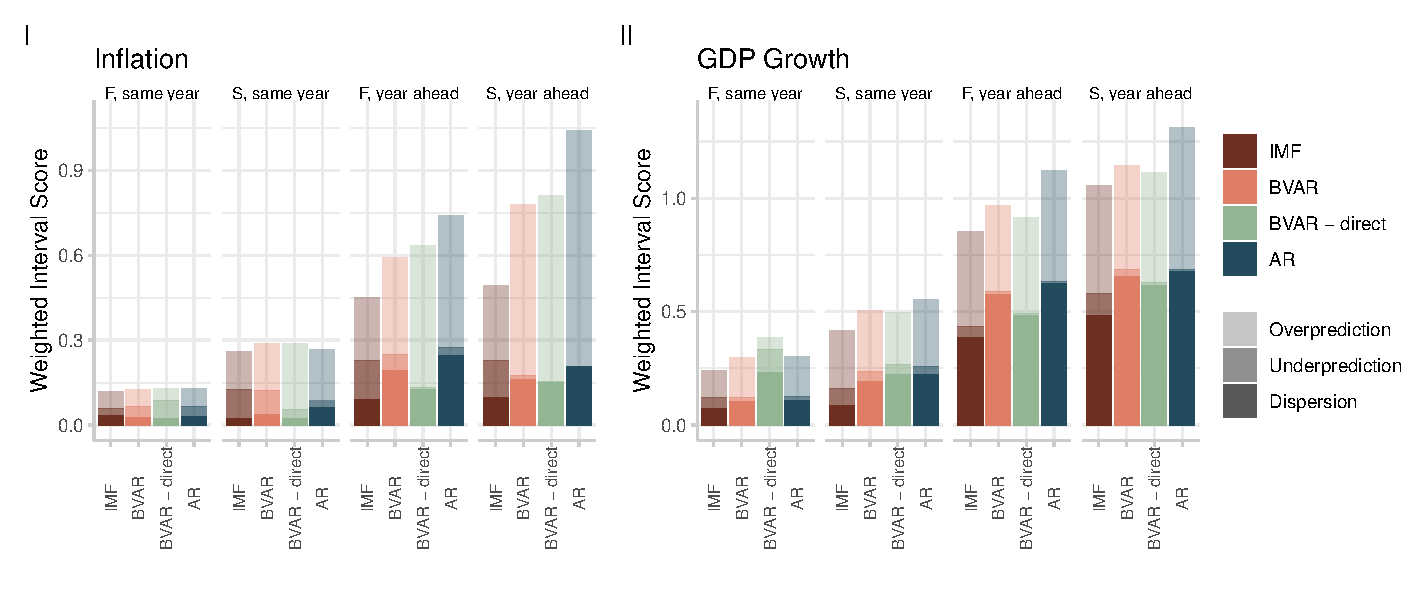
\includegraphics[width=0.95\textwidth]{figures/wis_cpigdp_new.pdf} 
        \label{fig:enter-label}
    \end{figure} 
\end{frame}

%\begin{frame}{Scores - Inflation}
%%    \begin{figure}
 %       \centering
 %       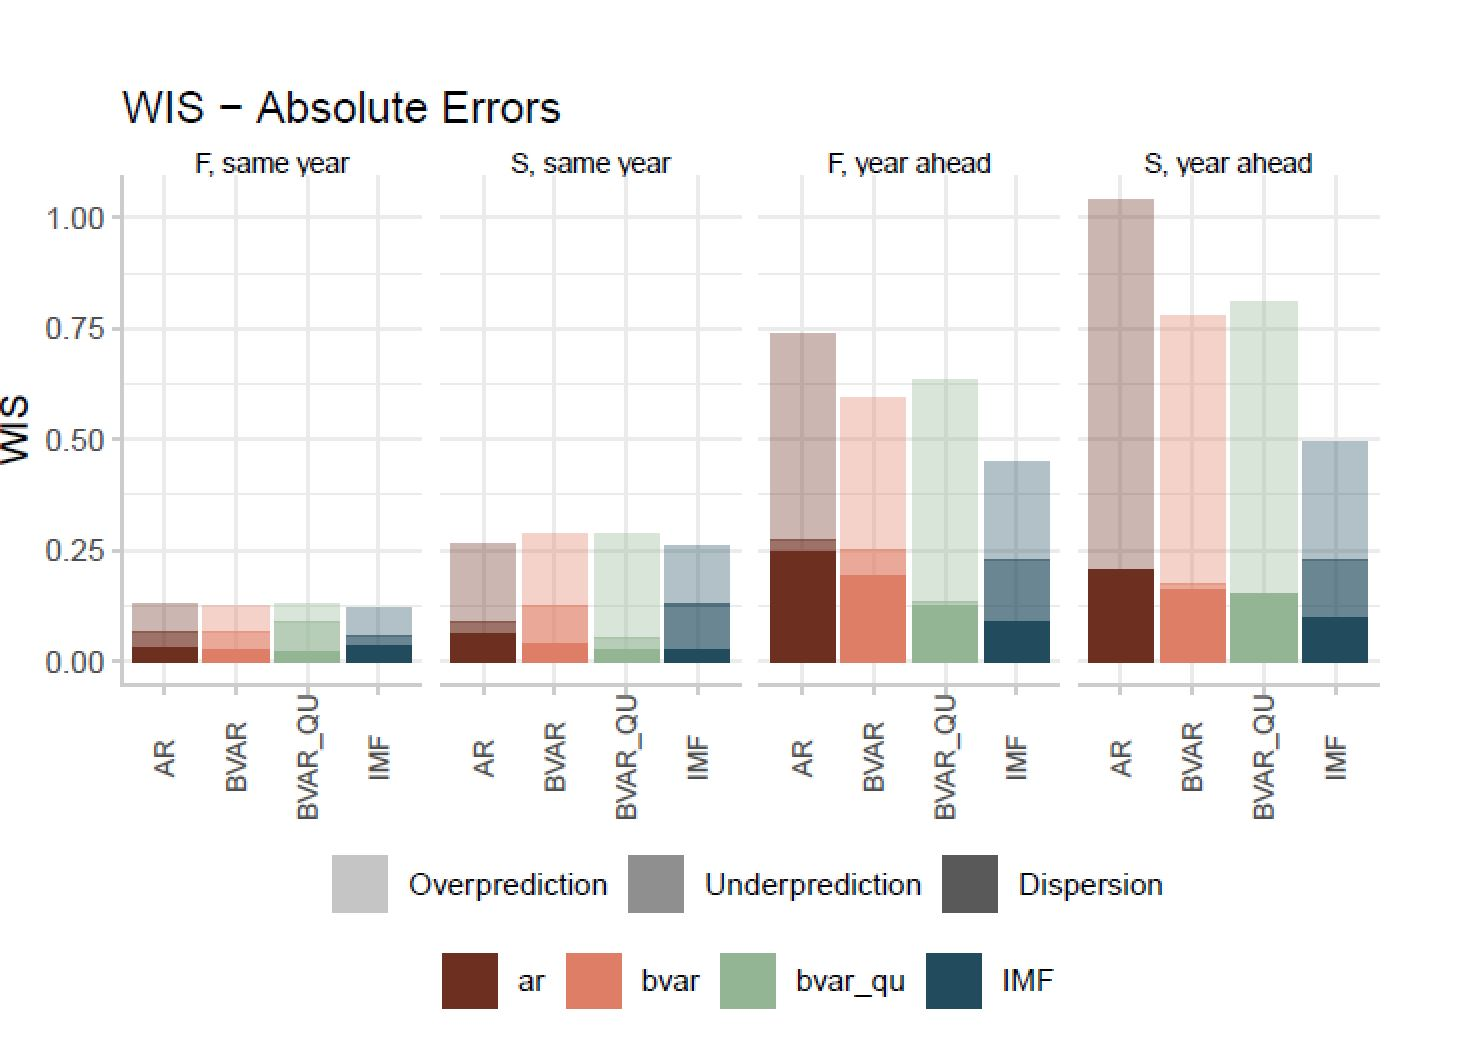
\includegraphics[width=0.45\textwidth]{figures/scores_absolute errors_cpi.JPG} 
 %       \label{fig:enter-label}
 %   \end{figure} 
%\end{frame}


\begin{frame}{Calibration - Interval Coverage Levels}
%\textit{Here, I'll instead map the colors to the different forecast sources (currently mapped to the window method), so we'll just have one plot each}
    %Coverage at the 50\% and 80\% central interval: \\ 
    \begin{figure}
        \centering
        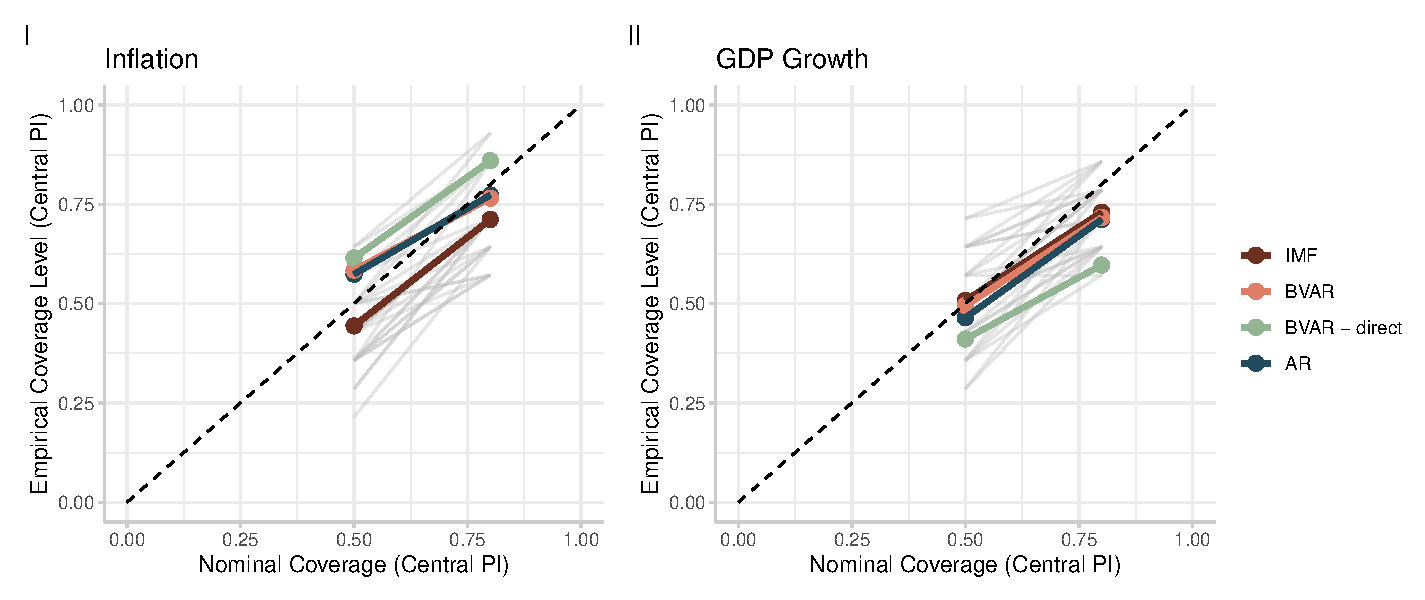
\includegraphics[width=0.9\textwidth]{figures/coverage.pdf}
        %\caption{Coverage at the 50 and 80 percent level}
        \label{fig:enter-label}
    \end{figure}
\end{frame}

\begin{frame}{Increasing Uncertainty}
%Width of Prediction Intervals, by Horizon
%\textit{include graphic or table showing increasing uncertainty with rising horizons}\\ 

\begin{columns}
\begin{column}{0.6\textwidth}
    \begin{figure}
        \centering
        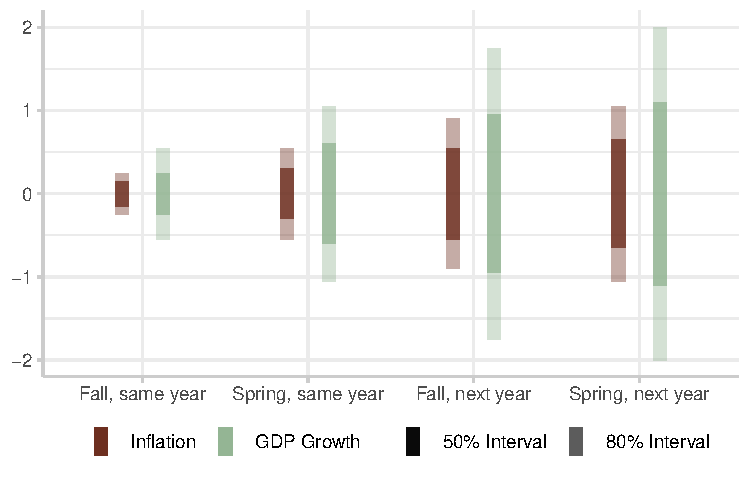
\includegraphics[width=\textwidth]{figures/horizon_uncc.pdf}
        %\caption{Coverage at the 50 and 80 percent level}
        \label{fig:enter-label}
    \end{figure}
\end{column}
\begin{column}{0.4\textwidth}
\centering
\textbf{Average length of intervals}
\begin{table}
\begin{tabular}{ l c c }
&   50\%  & 80\%\\[0.3em]
\multicolumn{3}{c}{\textbf{GDP Growth}}\\
Fall,  SY & 0.5 & 0.9\\ 
Spring, SY &0.8 &2.1 \\ 
Fall, NY & 2.2 & 3.9\\ 
Spring, NY &2.4 &4.9 \\[0.3em] 
\multicolumn{3}{c}{\textbf{Inflation}}\\
%&   50\%  & 80\%\\[0.3em]
Fall,  SY & 0.3 & 0.6\\ 
Spring, SY &0.5 &1.3 \\ 
Fall, NY & 1.2 & 2.2\\ 
Spring, NY &1.9 &2.4 \\ 
\end{tabular}
\end{table}
\vspace{1.25cm}
%\begin{table}
%\begin{tabular}{ l c c }
%\multicolumn{3}{c}{\textbf{Inflation}}\\
%%&   50\%  & 80\%\\[0.3em]
%Fall,  SY & 0.3 & 0.6\\ 
%Spring, SY &0.5 &1.3 \\ 
%Fall, NY & 1.2 & 2.2\\ 
%Spring, NY &1.9 &2.4 \\ 
%\end{tabular}
%\end{table}
\end{column}
\end{columns}


%\textit{relate back to article shown in the beginning, which also mentions IMF forecast of 0.1 percent $\rightarrow$ almost 50\% of any predictive intervals at this time would actually be below zero}
\end{frame}

\begin{frame}{Robustness Checks}
\textit{each will be linked to a short slide in Appendix giving the alternative results}
\begin{itemize}
    \item error extraction method: absolute vs. directional errors
    \item window method
    \item potential dependency of results on discretization \\
    \textit{what I mean by this: does the fact that we are extracting quantiles from the samples influence the results? Show results for sample-based CRPS}
\end{itemize}
\end{frame}



\section{Outlook}

\begin{frame}{Summing up}
\begin{itemize}
\item Attaching distributional forecasts via past forecast errors to an existing base of point forecasts is
    \begin{itemize}
        \item cheap
        \item competitive
        \item transparent
    \end{itemize}
\item Attachment of uncertainty to point forecasts is often substantial, making its communication necessary
\item IMF forecasts are valuable source for distributional forecasts in their own right \bigskip \\
\item     Outlook
    \begin{itemize}
        \item employ method that ideally utilizes the cross-section dimension, e.g. via Hierarchical Bayesian Modeling
    \end{itemize}

\end{itemize}
\end{frame}

\begin{frame}{Making it public}
\textit{Refer to Shiny App}    
\end{frame}

%\begin{frame}{Beispielinhalt: Literatur}
%    Literaturzitat: \cite{klare2021jss}
%end{frame}
%\begin{frame}
%        Bei Frames ohne Titel wird die Kopfzeile nicht angezeigt, und  
%    der freie Platz kann für Inhalte genutzt werden.
%\end{frame}

%\begin{frame}[plain]
%    Bei Frames mit Option \texttt{[plain]} werden weder Kopf- noch Fußzeile angezeigt.
%\end{frame}

%\begin{frame}[t]{Beispielinhalt}
%    Bei Frames mit Option \texttt{[t]} werden die Inhalte nicht vertikal zentriert, sondern an der Oberkante begonnen.
%\end{frame}

\appendix
\beginbackup

%\begin{frame}{Literatur}
%\begin{exampleblock}{Backup-Teil}
%    Folien, die nach \texttt{\textbackslash beginbackup} eingefügt werden, zählen nicht in die Gesamtzahl der Folien.
%\end{exampleblock}

%\printbibliography
%\end{frame}

%\section{Farben}
%% ----------------------------------------
%% | Test-Folie mit definierten Farben |
%% ----------------------------------------
%% ----------------------------------------
%% | /Test-Folie mit definierten Farben |
%% ----------------------------------------
\backupend

\end{document}